\pagebreak
\chapter{Algorithm of learning}
\label{chapter:Algorithm}

\section{Formulation of reinforcement learning}


Normally, reinforcement learning is formulated by a Markov decision process. The Markov decision process(MDP) means that
It models Agents that make decisions and is formulated as a set of four with the following elements.
\begin{itembox}[l]{Markov decision model}
\bm{State:} \hspace{1.2cm} $S = \{ s^{(1)}, s^{(2)}, ... , s^{(N)} \}$

\bm{Action:} \hspace{1cm} $A = \{ a^{(1)}, a^{(2)}, ... , a^{(K)} \}$ 

\bm{Dynamics:} \hspace{5mm} $T : S \times A \times S \rightarrow [0, 1]$ \hspace{1cm} $T(s',a,s) = p(s' | s,a)$

\bm{Reward:} \hspace{0.9cm} $R : S \times A \times S \rightarrow \mathbb{R}$
\end{itembox}

Here, Dynamics is a state transition function.
Reward $R(s, a, s')$ represents the immediate reward obtained when transitioning from state $s$ to $s′$ with action, or the expected value $\mathbb{E}[r_{t+1}|s,a,s']$.
Here, the expected value of the immediate reward is defined as a reward function $r(s, a)$.

The time series of the state of a certain agent is expressed as $S_t = \{s_1, ... , s_t \}$, and the action series is expressed as $A_{t-1} = \{ a_1, ..., a_{t-1} \}$.
At this time, the trajectory of the Agent is a series of pairs of “state” and “action” represented as $\bm{\zeta} = \{ (s_1, a_1), ... , (s_t, a_t) \}$.

Here, consider a grid world like as a following one-person game,  shown in figure\ref{fig:example_gridworld}. The robot moves and gets +1 when reaching the treasure and -1 when reaching the bomb.
In this simple world, the environment and the robot interact. If this world is represented by a Markov decision model, state $S$ is the position of the robot, and action $A$ is the action that the robot can take, that is, up, down, right, and left.
The reward for reaching the jewel is +1 and the reward for reaching the bomb is -1.
For example, reward function $R(s, a) = -1$ for an right action $a$  where the robot is at the left position $s$ of the bomb.


\begin{figure}[H]
\begin{center}
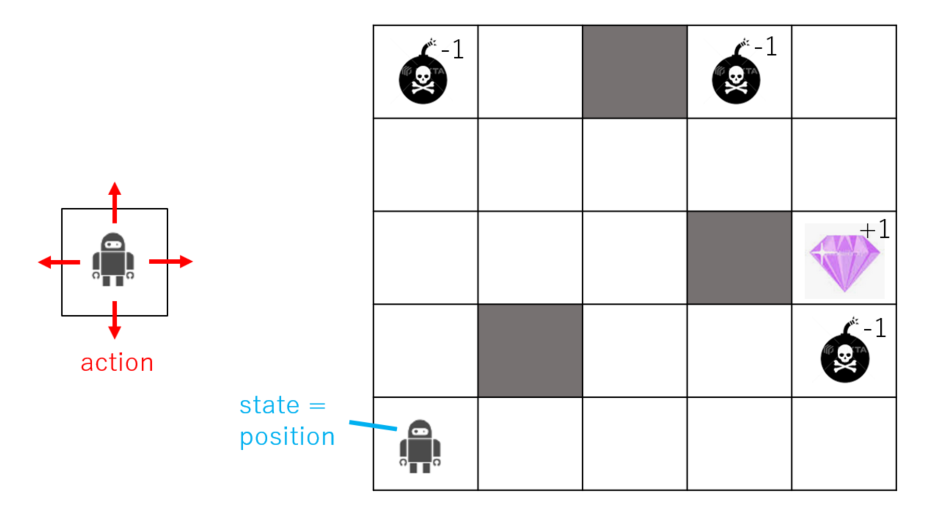
\includegraphics[width=14cm]{./figures/example_gridworld.png}
\caption{Grid world.}
\label{fig:example_gridworld}
\end{center}
\end{figure}

A Markov process that depends on a state in the past by one unit time is called a simple Markov process, and a Markov process that depends on a past state in more than two unit times is called a multiple Markov process. On the other hand, Markov processes that are not bound by past states are called homogeneous Markov processes. Here we concentrate on the homogeneous Markov process.


\subsection{Reinforcement learning problem formulation}

The problem of reinforcement learning can be formulated as a problem such that to find the optimal policy $\pi^{*}$ that maximizes the expected value of the time sum of rewards $R = \sum_{t'} \gamma^{t'} r_{t'+1}$ in the probability distribution $\pi(a|S_t,A_{t-1})$ that selects actions $a_t$ based on the realization values ​​of state time series $S_t = \{ s_1, ... , s_t\}$ and action time series $A_t = \{ a_1, ... , a_{t-1}\}$.

Here, $\gamma$ is the discount factor satisfying $0\leq \ \gamma \ \leq \ 1$, which is usually close to 1. (For example, $\gamma =1/(1+r)$ for some discount rate r.)
When the discount rate is applied, the sum of past rewards is evaluated lower than the latest reward.f the discount rate is not used, the sum of the rewards may diverge.

If dynamics of Markov decision process is homogeneous, then optimal homogeneous policy also exists.
If Markov model is homogeneous, the trajectory of the Agent $\bm{\zeta} = \{ (s_1, a_1), ... , (s_t, a_t) \}$ is generated by homogeneous dynamics $p(s'|s,a)$ and homogeneous policy$\pi(a|s)$.  


\section{Introduction and formulation of generative adversarial imitation learning}

\subsection{Introduction of TRPO}

Now writing ...

\begin{itemize}
\item policy optimization
\item advantage function
\end{itemize}


\subsection{Introduction of GAIL}

Now writing ...

\begin{itemize}
\item adversarial network
\item policy network
\item surrogate reward
\item objective of GAIL
\end{itemize}


